\chapter[The Magic-sets Rewrite]{The Magic-sets Rewrite}
\label{ch:magic}

Having described the Evita Raced infrastructure, we now turn to our use of it
to specify query optimizations in \OVERLOG.  Using Evita Raced, we have
developed three optimization techniques from the literature: the magic-sets
rewrite~\cite{magic-sets1, magic-sets2}, the System R dynamic
program~\cite{selinger} and the Cascades branch-and-bound
algorithm~\cite{cascades}.  In this chapter, we describe the magic-sets
rewrite, developed as a declarative compiler stage for Evita Raced.  The
problem address by magic-sets is that often a query in a program does not ask
for the entire relation.  For example, the \ol{path} query in
Figure~\ref{ch:p2:fig:overlogSP} asks for the subset of paths that originate
from ``node1.'' In order to efficiently answer such a query, the
magic-sets rewrite pushes query constants down into the rules so that a Datalog
evaluator {\emph never} derives facts that do not contribute to the query.

Datalog-oriented systems like P2 perform a bottom-up (\emph{forward chaining})
evaluation on each rule, starting with known facts (tuples), and recursively
deriving new facts through rule deductions.  The advantage of this strategy is
that the evaluation is data driven (from known facts to possible deductions)
and will not enter infinite loops for some statically verifiable \emph{safe}
programs.  In contrast, top-down (\emph{backward chaining}) evaluation (e.g.,
in the Prolog language), starts with the query predicates as the top-level
goals, and recursively identifies rules whose head predicates unify with needed
goals, replacing them with the subgoal predicates in the rule body, until all
subgoals are satisfied by known facts or rejected when no further recursion is
possible.  The advantage of a top-down evaluation strategy is that it avoids
resolving goals that are not needed by the posed queries.

At a high-level, the magic-sets rewrite performs a transitive closure, on the
rules of a Datalog program, to obtain extra predicates that prune results,
known to be superfluous, from a bottom-up evaluation.  The primary data
structure used by this rewrite technique is a rule/goal graph, which we review
in Section~\ref{ch:magic:sec:review}, along with the magic-sets algorithm.
Using the rule/goal graph representation of an \OVERLOG program, in
Section~\ref{ch:magic:sec:rules} we express the magic-sets rewrite in $44$ 
\OVERLOG rules.  We divide these rules into two logical groups.  The first is
presented in Section~\ref{ch:magic:sec:rgconstruct}, which constructs the
rule/goal graph via a transitive closure on the Metacompiler Catalog.  Our
second group of rules, presented in Section~\ref{ch:magic:sec:rewrite}, express
a transitive closure on the rule/goal graph, to obtain the rewritten rules that
include new predicates that filter tuples that do not contribute to the query
result.

\section{Magic-sets in a Nutshell}
\label{ch:magic:sec:review}

\begin{figure*}[!t]
\ssp
\centering
\begin{boxedminipage}{\linewidth}
{\bf link}(``node1'', ``node2'', 1).\\
{\bf link}(``node1'', ``node3'', 1).\\
{\bf link}(``node2'', ``node1'', 1).\\
...\\
r1 {\bf path}(@X, Y, P, C) :- \\
\datalogspace {\bf link}(@X, Y, C), P := f\_cons(X, Y). \\
\\
r2 {\bf path}(@X, Z, P, C) :- \\
\datalogspace {\bf link}(@X, Y, C1), {\bf path}(@Y, Z, P2, C2),\\
\datalogspace f\_contains(X, P2) == false, \\
\datalogspace P := f\_cons(X, P2), C := C1 + C2. \\
\\
Query: path(@LOCALHOST, Y, P, C).
\end{boxedminipage}
\caption{\label{ch:magic:fig:basicSP}The path-only rules copied from Figure~\ref{ch:p2:fig:overlogSP}.}
\end{figure*}

\begin{figure*}
\centering

\includegraphics[scale=1.2]{figures/Topology}
\caption{Experimental topology.}
\label{ch:evita:fig:topo}
\end{figure*}

The magic-sets technique rewrites logical rules so that bottom-up evaluation
over the rewritten rules has all advantages of both top-down and bottom-up
strategies.  We review the main advantages here by example using the path
program shown in Figure~\ref{ch:magic:fig:basicSP}.  For the purposes of this
discussion, lets assume we execute these rules locally with the initial set of
link facts forming the topology shown in Figure~\ref{ch:evita:fig:topo}.  The
abbreviated list of facts shown at the beginning of
Figure~\ref{ch:magic:fig:basicSP} populate the \ol{link} relation with our
basic topology information.  Our goal is to find all paths that start at
@LOCALHOST, which for this example we will assume this is $node1$.

A straightforward bottom-up evaluation of this program applies the \ol{link}
tuples to rule \ol{r1}, creating the initial set of {\tt path} tuples.  Rule
\ol{r2} performs a transitive closure over the \ol{link} and \ol{path}
relations, while any \ol{path} tuples matching ``node1'' on their first
attribute are returned in the programmer's query.  Clearly this bottom-up
evaluation strategy examines some \ol{path} tuples at the query level for
matches with ``node1'' along the first attribute.  In contrast, a top-down
evaluation begins by unifying the query predicate with the head predicate of
rules \ol{r1} and \ol{r2}.  This \ol{path} predicate unification binds the $@X$
attribute to ``node1'' in both rules, which is then carried over to the
predicates in the rule body.  Binding $@X$ in rules \ol{r1} and \ol{r2}
effectively means that these rules will only look for tuples of the form
\ol{path(``node1'', Y, P, C)}, and nothing else.

The magic-sets rewrite is an optimization that can accomplish the same
efficiency found in the top-down evaluation, using a bottom-up evaluator.
Since it is still bottom-up, we retain all the benefits of seminaive
evaluation: set-oriented evaluations, unique minimal model and stratification.
It does this by adding extra selection predicates to the rules of a program to
emulate the goal-oriented execution of top-down evaluation (sometimes called
\emph{sideways information passing} or SIP).  Conceptually, given a rule of the
form $H\ \text{\ol{:-}}\ G_1, G_2, ..., G_k$, where $H$ is the head predicate
and $G_{1,...,k}$ are the subgoals, the magic-sets rewrite intersperses
selection predicates $s_{1,...,k}$ to generate the rule form $H\
\text{\ol{:-}}\ s_1, G_1, s_2, G_2, ..., s_{k}, G_k$.  Facts for these
selection predicates are generated according to attribute bindings, in the
user's query or from other rule predicates in the program, to constant values.

\begin{figure*}[!t]
\ssp
\begin{boxedminipage}{\linewidth}
{\bf link}(``node1'', ``node2'', 1).\\
{\bf link}(``node1'', ``node3'', 1).\\
{\bf link}(``node2'', ``node1'', 1).\\
...\\
{\bf magic\_path}(``node1''). \\
\\
r1\_case5 {\bf path}(@X, Y, P, C) :- \\
\datalogspace {\bf magic\_path}(@X), \\
\datalogspace {\bf link}(@X, Y, C), P := f\_cons(X, Y).\\

r2\_case2 {\bf sup\_r2\_1}(@X, Y, C1) :- \\
\datalogspace {\bf magic\_path}(@X), \\
\datalogspace {\bf link}(@X, Y, C1). \\

r2\_case3 {\bf magic\_path}(@Y) :- \\
\datalogspace {\bf sup\_r2\_1}(@X, Y, C1). \\

r2\_case4 {\bf sup\_r2\_2}(@X, Y, Z, C1, P2, C2) :- \\
\datalogspace {\bf sup\_r2\_1}(@X, Y, C1), \\
\datalogspace {\bf path}(@Y, Z, P2, C2). \\

r2\_case5 {\bf path}(@X, Z, P, C) :- \\
\datalogspace {\bf sup\_r2\_2}(@X, Y, Z, C1, P2, C2), \\
\datalogspace f\_contains(X, P2) == false, \\
\datalogspace P := f\_cons(X, P2), C := C1 + C2. \\

Query: {\bf path}(``node1'', Y, P, C).
\end{boxedminipage}
\caption{\label{ch:magic:fig:magicSP}A magic-sets rewrite of 
the rules in Figure~\ref{ch:magic:fig:basicSP}.}
\end{figure*}

Figure~\ref{ch:magic:fig:magicSP} shows the rewritten rules from the path
program in Figure~\ref{ch:magic:fig:basicSP}.  The program contains a some new
predicates mixed in to some rules that feed those predicates with tuples, and
some that ``join'' old predicates to these new predicates.  Ullman refers to
these new predicates as magic predicates (i.e., \ol{magic\_path}) and
supplementary predicates (i.e., \ol{sup\_r2\_1}, \ol{sup\_r2\_2}).  Magic predicates
maintain bindings for the final query predicate, while supplementary predicates
pass bindings along rule bodies, ensuring that no extraneous deductions are made.

We now describe the rewritten rules, which are named by the original rule
follows by a ``case'' number that will be described in
Section~\ref{ch:magic:sec:rewrite}.  In case 1, we create a single fact for the
magic predicate \ol{magic\_path} that contains the bound constants from the
query predicate.  Lets start by looking at rule~\ol{r1}, again assuming we are
running locally with all facts in the \ol{link} relation, and a query predicate
asking for ``node1''.  If at this point, rule~\ol{r1} where to derive a \ol{path}
from any \ol{link} fact, other than those that originate from ``node1'', then
it would be incorrect.  To avoid this occurrence, we add the \ol{magic\_path}
predicate to the body of the rule giving us rule~\ol{r1\_case5}.

Rule~\ol{r2} appears to be quite a bit more complicated, expanding out to
four separate rules. We describe the purpose of each rule on a case-by-case
basis. Rule~\ol{r2\_case2} adds a rule that fills the \ol{sup\_r2\_1} relation
with tuples produced by ``joining'' \ol{magic\_path} and \ol{link} relations.
The outcome of which is no different then rule~\ol{r1\_case5} in our previous 
discussion. The interesting bit here is that the tuples in \ol{sup\_r2\_1} 
feed into a ``join with'' the \ol{path} predicate in rule~\ol{r2}. By pruning
tuples, using \ol{magic\_path}, from this result set before considering the
\ol{path} relation, we avoid generating superfluous tuples. 

This brings us to the more interesting case~$3$ from rule~\ol{r2}. Here we are
feeding the \ol{sup\_r2\_1} tuples into the \ol{magic\_path} predicate. The
reason is that whatever tuples are considered by the \ol{path} relation are
required in order to answer the query. We indicate this by adding new binding
constants, that do not necessarily equate to ``node1.'' In fact, throughout
this evaluation, the \ol{magic\_path} relation will be given constant values
for each node name in the topology because there is a path from node 1 to it.
This action seen by noticing that rule~\ol{r2\_case3} feeds the $Y$ variable
to the \ol{magic\_path} relation.

The remaining cases simply stitch things up in the remainder of rule~\ol{r2}.
In case~$4$, we combine \ol{sup\_r2\_1} with the \ol{path} predicate to obtain
the \ol{sup\_r2\_2}, which is then used to finish off the rule in case~$5$
(rule~\ol{r2\_case5}).  The reader may be confused by the need for
\ol{sup\_r2\_2}.  Consider the reasoning for all these extra cases when dealing
with rule~\ol{r2}.  Rule~\ol{r2} contains the \ol{path} predicate, which is
also the query predicate.  This triggered the extra steps taken beyond the
simple case~$5$ for rule~\ol{r1}.  The point is that the \ol{path} predicate
could occur many times in a rule body, and each time we need to initiate cases
$2-4$.  On subsequent steps, we need to consider the supplementary predicate
that followed the previous instance of the \ol{path} predicate.  That is the
purpose of \ol{sup\_r2\_2}, but in this case we only had the one \ol{path}
subgoal.

Before we can present the declarative rules for implementing this rewrite
technique, we must review the concept of adornments and the rule/goal graph
representation for a collection of Datalog (\OVERLOG) rules.  These data
structures form the basis of the transitive closure algorithm performed by the
magic-sets rewrite, and our declarative rules follow this model.  The
discussion leading up to Section~\ref{ch:magic:sec:rules} follows from
Chapter~$13$ of Ullman's textbook~\ol{ullmanTextbook}, which provides the most
through coverage on the subject to date.


\subsection{Adornments}

Consider again a snippet of the shortest path program in
Figure~\ref{ch:magic:fig:basicSP}.  The query predicate \ol{path(``node1'', Y,
P, C)} asks for the shortest path from all nodes to node ``node1''.  We can
indicate which path arguments are bound and which are free by an {\emph
adornment}, which is a binding pattern that contains a string of {\emph b's}
and {\emph f's} of length {\emph k}, for each {\emph k} arguments of path.  In
the current context, the {\emph path} query predicate has a $path^{bfff}$
adornment since the first argument is bound to a constant and the last three
are free variables.

Each rule in an \OVERLOG program is also given an adornment according its
left-to-right evaluation order.  The steps for assigning rule adornments are as
follows.
\begin{enumerate}
    \ssp
    \item A variable appearing in a bound argument of the rule head is bound before processing any subgoals.
    \item A variable is bound after processing subgoal $G_i$ if it was bound 
          before processing $G_i$ or if it appears anywhere in $G_i$.
\end{enumerate}
The format of a rule adornment differs from that of a predicate.  It follows the form
$[B_1,\cdots,B_m|F_1,\cdots,F_n]$, which contains two sublists of variables
separated by a bar.  The variables to the left of the bar (i.e.,
$B_1,\cdots,B_m$) represent bound variables, while those to the right (i.e.,
$F_1,\cdots,F_n$) are free. 

A given rule contains a number of these binding patterns, one for each subgoal
position.  A rule adornment is a binding pattern of a rule at a particular
position.  The notation that we follow here for rule adornments identifies the
rule's position as a subscript and the binding pattern as a superscript.  For
example, $r1_0^{[@X|Y,P,C]}$ is the adornment for rule \ol{r1} at the head
position $0$, which taken from the binding pattern of the query (goal)
predicate adornment $path^{bfff}$.  Continuing, $r2_0^{[@X,|Y,Z,C1,P,C]}$
represents the adornment for rule~\ol{r2} at the head position $0$, again
binding the first variable of the head predicate.  This rule adornment creates
the new $link^{bff}$ adornment for the \ol{link} subgoal.  The \ol{link}
predicate adds variables $Y$ and $C1$ to the list of bound variables at the
rule position $1$.  This gives us the $r1_1^{[@X,Y,C1,|Z,P,C]}$ rule adornment,
which will feed bindings into the \ol{path} predicate, feeding the same
$path^{bfff}$ adornment with its binding of the $Y$ variable.

\subsection{Rule/Goal Graphs}

\begin{figure*}[!t]
\begin{center}
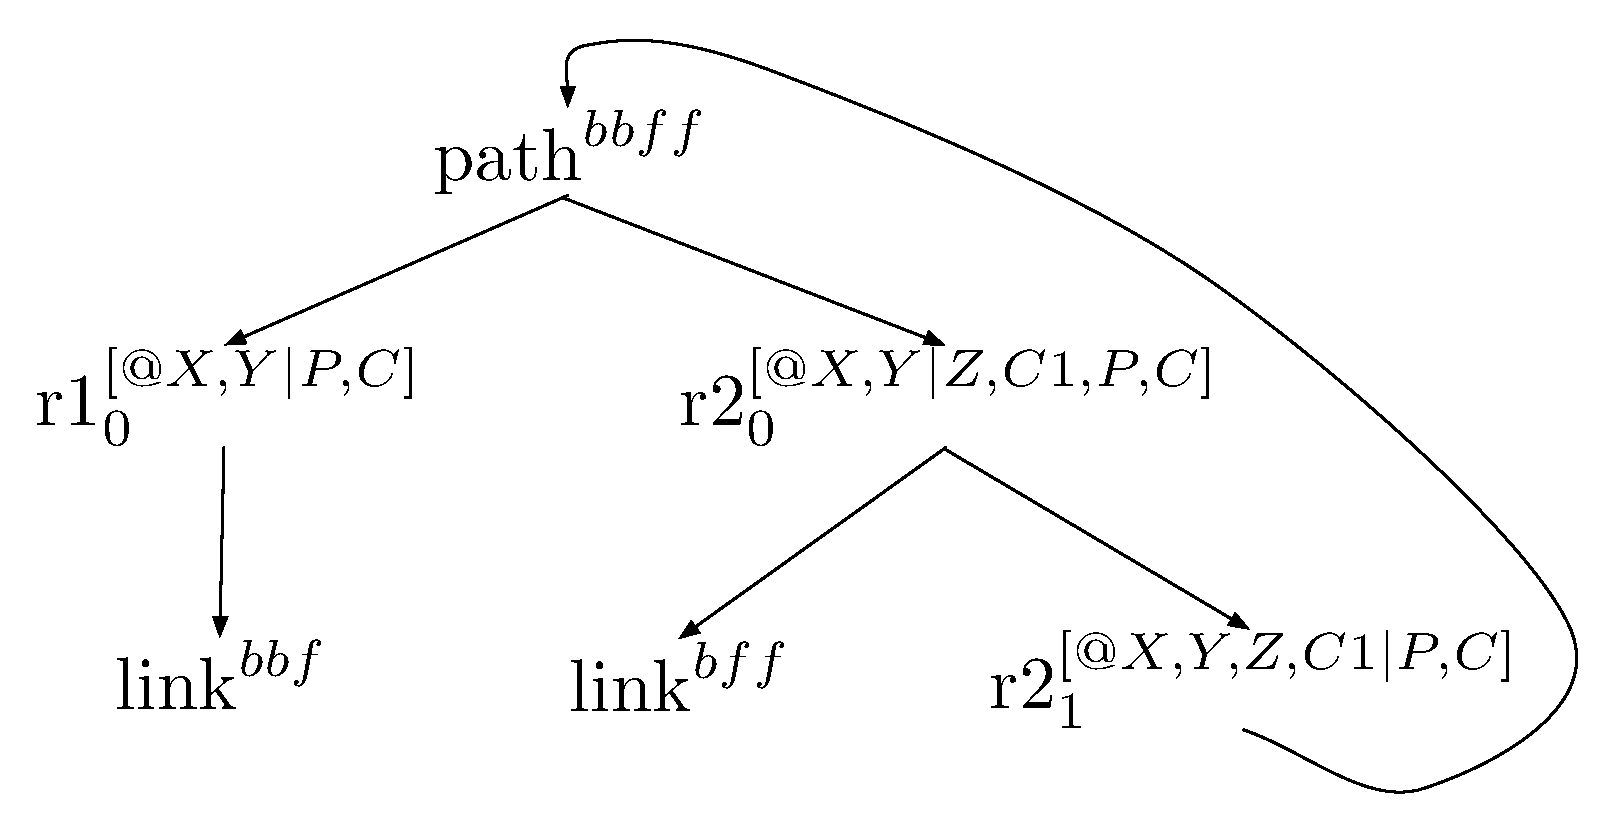
\includegraphics[scale=0.5]{figures/RuleGoalGraph}
\caption{\label{ch:magic:fig:rggraph}Rule/Goal graph of the program in Figure~\ref{ch:magic:fig:basicSP}.}
\end{center}
\end{figure*}

A rule/goal graph the a representation of binding patterns that occur in a
collection of Datalog (\OVERLOG) rules.  The graph consists of \emph{rule} and
\emph{goal} vertices.  A goal vertex consists of a predicate with an adornment
(e.g., $path^{bfff}$) and similarly, a rule vertex represents the adornment of
the rule in a particular position (e.g., $r1_0^{[@X|Y,P,C]}$).

Figure~\ref{ch:magic:fig:rggraph} illustrates the {\em rule/goal} graph for our
Figure~\ref{ch:magic:fig:basicSP} example.  To construct this graph, we start
at the query predicate, and creates a goal vertex in the graph with the
appropriate adornment.  For every rule with that goal predicate as its head, we
create a position $0$ rule adornment.  For rule~\ol{r1} this is
$r1_0^{[@X|Y,P,C]}$ and for rule~\ol{r2} we have $r2_0^{[@X,|Y,Z,C1,P,C]}$.  A
rule vertex feeds bindings to the subgoal just beyond its position and the rule
position subsequent to its own.  Both rules in position $0$ bind the \ol{link}
predicate variable $X$.  In the case of rule~\ol{r2}, rule position~$1$
receives the bindings of its parent rule and from the \ol{link} child subgoal,
giving us the $r1_1^{[@X,Y,C1,|Z,P,C]}$ rule vertex.

At this point in rule~\ol{r2} we have reached the position prior to the
\ol{path} predicate.  We create the appropriate $path^{bfff}$ adornment, which
matches up with our original \ol{path} goal node.  Since we have not further
rule binding steps beyond the path predicate, the process halts.  Our
declarative rules, described next, initiate the rewrite process by performing
these steps in a transitive closure over the Metacompiler Catalog.

\section{Declarative Magic-sets}
\label{ch:magic:sec:rules}

Using Evita Raced, we expressed the magic-sets rewrite stage in \OVERLOG.  Our
\OVERLOG rules that perform the rewrite are based on the description in the
previous section, which follows Ullman's textbook
description~\cite{ullmanTextbook}.  The first step in this algorithm constructs
the rule/goal graph, captured as data in a set of relations.  It uses this
graph data to check for the {\emph unique binding property} with respect to the
adornment of the query predicate.  This property is met when the query
predicate $q_p$, expressed against predicate $p$, contains a unique ``binding
pattern'' throughout the rule/goal graph.  The query predicate $q_p$ provides
the first binding patterns (the root of the rule/goal graph), while rules that
mention $p$ further bindings based on sideways-information-passing (SIP).

We check for the unique binding property in the first phase of our rewrite,
while constructing the rule/goal graph through a transitive closure over the
Metacompiler Catalog.  The Metacompiler Catalog already provides some of the
rule/goal graph information, specifically goal (head predicate) and subgoal
(body terms) rule dependencies.  The remaining information that we need to
collect is the adornment information for goal and rule ``vertices.''  Once this
information is secured, we can move to the actual rewrite rules
described in Section~\ref{ch:magic:sec:rewrite}, where magic and supplementary
relations are created according to the five cases previously discussed.

\subsection{Rule/Goal Graph Construction}
\label{ch:magic:sec:rgconstruct}

The algorithm for constructing a rule/goal graph begins at the query
predicate, and recursively through the rules that mention the query predicate
in the head.  We assume the unique binding property holds in the beginning, and
detect if it does not along the way.  Techniques exists for rewriting a program
so that the unique binding property always holds but we did not consider that
in this work.  Given a query predicate $q_p$, we assign a {\emph magic predicate}
denoted as $m_p$ with a corresponding adornment.  A set of {\emph supplementary
predicates}, denoted as $sup_i$ ($i$ being the rule position), are also created as
we recursively walk the rules in a left-to-right (SIP) order.


\begin{figure*}[!t]
\ssp
\centering
\begin{boxedminipage}{\linewidth}

/* Create an adornment for the query predicate and add a fact to the \\
\ol{magicPred} table referencing this adornment. */ \\
ms1 {\bf magicPred}(@A, Pid, Name, Sig) :- \\
\datalogspace {\bf magic::programEvent}(@A, Pid, ...), \\
\datalogspace {\bf sys::rule}(@A, Rid, Pid, ... , Goals), \\
\datalogspace {\bf sys::predicate}(@A, \_, Rid, ..., Schema), \\
\datalogspace $Goals == 1$, \\
\datalogspace Sig := f\_adornment(Schema).
	
\end{boxedminipage}
\caption{\label{ch:magic:fig:magic1}Construction of the query adornment and corresponding magic predicate.}
\end{figure*}

The abbreviated rule in Figure~\ref{ch:magic:fig:magic1} creates an adornment
for the query predicate and adds that fact to the \ol{magicPred} relation.  A
query predicate is identified in P2 by a rule containing a single goal ($Goals
== 1$).  The sole predicate in this rule has a schema ($Schema$) that contains
some number of (binding) constants and (free) variables.  The function {\emph
f\_adornment} takes such a schema object as its argument and returns a string
representing the adornment signature.

The previous rule (\ol{ms1}) created the top-level goal node, which is the root
of the rule/goal graph.  The group of rules in Figure~\ref{ch:magic:fig:magic2}
deal with creating adornments for rule positions in the target program.  We
store the rule adornment in a \ol{sup} relation since this information will be
used to create supplementary predicates in Section~\ref{ch:magic:sec:rewrite}.
A \ol{sup} tuple contains the following attributes in order:
\begin{itemize}
   \ssp
  \item A reference to the target program and rule identifiers. 
  \item The position within that target rule.
  \item A name for the supplementary predicate.
  \item A rule adornment, as schema object containing all constants and variables up to that rule position.
  \item A new identifier that will be used (in Section~\ref{ch:magic:sec:rewrite}) to create 
    a new rule that supplies facts to the supplementary relation (e.g., rule cases $2$ and $4$ 
    in Figure~\ref{ch:magic:fig:magicSP}).
\end{itemize}

\begin{figure*}[!t]
\ssp
\centering
\begin{boxedminipage}{\linewidth}
/* Initialize sup position 0 for rules that reference a magic predicate in the head. */ \\
ms2 {\bf sup}(@A, Pid, Rid, Pos, SupName, Schema, f\_idgen()) :- \\
\datalogspace {\bf magicPred}(@A, Pid, Name, Sig), \\
\datalogspace {\bf sys::rule}(@A, Rid, Pid, RName, HeadPid, ...), \\
\datalogspace {\bf sys::predicate}(@A, HeadPid, Rid, \_, Name, ..., FSchema, ...), \\
\datalogspace Schema := f\_project(Sig, FSchema), \\
\datalogspace SupName := "sup\_" + RName + 0, \\
\datalogspace Pos := 0. \\

/* Create supplementary predicate for a given subgoal. */ \\
ms3 {\bf sup}(@A, Pid, Rid, Pos, SupName, NewSchema, f\_idgen()) :- \\
\datalogspace {\bf supNext}(@A, Pid, Rid, Pos, Schema), \\
\datalogspace {\bf sys::rule}(@A, Rid, Pid, RName, ...), \\
\datalogspace {\bf sys::predicate}(@A, Fid, Rid, ..., FSchema, Pos, ...), \\
\datalogspace SupName := "sup\_" + RName + "\_" + Pos, \\
\datalogspace NewSchema := f\_merge(Schema, FSchema). \\
	
/* Create supplementary predicate for a given assignment. */ \\
ms4 {\bf sup}(@A, Pid, Rid, Pos, SupName, NewSchema, f\_idgen()) :- \\
\datalogspace {\bf supNext}(@A, Pid, Rid, Pos, Schema), \\
\datalogspace {\bf sys::rule}(@A, Rid, Pid, RName, ...), \\
\datalogspace {\bf sys::assign}(@A, Aid, Rid, Var, \_, Pos), \\
\datalogspace SupName := "sup\_" + RName + "\_" + Pos, \\
\datalogspace NewSchema := f\_assignschema(Schema, Var). \\ 

/* Move the rule position forward when update occurs to sup. */ \\
ms5 {\bf supNext}(@A, Pid, Rid, Pos+1, Schema) :- \\
\datalogspace {\bf sup}(@A, Pid, Rid, Pos, Name, Schema, Tid). \\
	
/* Move supNext forward for selection predicates. */ \\
ms6 {\bf supNext}(@A, Pid, Rid, Pos+1, Schema) :- \\
\datalogspace {\bf supNext}(@A, Pid, Rid, Pos, Schema), \\
\datalogspace {\bf sys::rule}(@A, Rid, Pid, ..., Goals), \\
\datalogspace {\bf sys::select}(@A, Sid, Rid, \_, Pos, \_), \\
\datalogspace $Pos < Goals$. 
\end{boxedminipage}
\caption{\label{ch:magic:fig:magic2}Rules for supplementary relational predicates.}
\end{figure*}

We now describe the details of each rule in Figure~\ref{ch:magic:fig:magic2}.
Rule~\ol{ms2} initiates the first \ol{sup} deduction.  It joins \ol{magicPred}
with the \ol{rule} and \ol{predicate} relations to obtain those rules that
contain the magic predicate in the head.  This result will represent the
supplementary predicate in position~$0$.  The adornment for this rule position
is obtained by projecting the head predicate schema onto the magic predicate
adornment.  The function {\emph f\_project} takes care of the step-by-step
details of combining the head predicate schema and the signature of the magic
predicate adornment, then returning a new schema that contains only the bound
head variables (according to the adornment).  For example, if the head
predicate schema is $[@X, Y, P, C]$ and the adornment is $bfff$ then the {\emph
f\_project} would return $[@X]$ as the new schema.  This new schema will be the
schema for the current supplementary predicate.

The rules that receive a \ol{sup} tuple are consider next by creating further
\ol{sup} tuples for each subgoal position.  In \OVERLOG, table predicates and
assignment statements create new bindings.  As a result, \ol{sup} tuples are
only generated for rule positions relevant to such terms: relational predicates
(rule~\ol{ms3}) and assignment statements (rule~\ol{ms4}).  The {\emph
f\_merge} and {\emph f\_assignschema} functions are used to update the schema
object with the bindings of the current term position.  A series of
\ol{supNext} tuples identify a rule position that is to be considered.  The
\ol{supNext} relation is updated in rule~\ol{ms5} for predicate and assignment
terms, rule~\ol{ms6} for selection predicate terms, which add no bindings to
the previous schema.


\begin{figure*}[!t]
\ssp
\centering
\begin{boxedminipage}{\linewidth}
/* We've encountered a magic predicate in the body of a rule. \\
   Compute its adornment based on current bound variables. */ \\
ms7 {\bf magicPred}(@A, Pid, FName, Sig) :- \\
\datalogspace {\bf supNext}(@A, Pid, Rid, Pos, Schema), \\
\datalogspace {\bf sys::rule}(@A, Rid, Pid, RName, ...), \\
\datalogspace {\bf sys::predicate}(@A, Fid, Rid, \_, FName, ..., FSchema, Pos, ...), \\
\datalogspace {\bf magicPred}(@A, Pid, FName, Sig), \\
\datalogspace Sig := f\_adornment(Schema, FSchema).

\end{boxedminipage}
\caption{\label{ch:magic:fig:magic3}Encountering a magic predicate during subgoal traversal.}
\end{figure*}

The previous group of rules ignored the special case of discovering a magic
predicate at the position in the \ol{supNext} tuple.  In order to verify that
the unique binding property holds, we must compute the adornment for the magic
predicate based on the bindings at given position.
Figure~\ref{ch:magic:fig:magic3} contains the single rule that generates a new
adornment for a subgoal that happens to be a magic predicate.  If the adornment
is different than the previous, then multiple rows will exist in the
\ol{magicPred} relation, signaling the presence of multiple adornments (the
primary key does not cover the adornment attribute).  A simple count query can
then be used to detect unique binding property violations.  This constraint
rule appears next in Figure~\ref{ch:magic:fig:magic4}.

\begin{figure*}[!t]
\ssp
\centering
\begin{boxedminipage}{\linewidth}
/* Indicate when a rule has been fully explored. */ \\
ms9 {\bf ruleComplete}(@A, Pid, Rid) :- \\
\datalogspace {\bf supNext}(@A, Pid, Rid, Pos, \_), \\
\datalogspace {\bf sys::rule}(@A, Rid, Pid, ..., Goals), \\
\datalogspace $Pos == Goals$. \\
	       
/* Count the number of completed rules. */ \\
ms10 {\bf rulesComplete}(@A, Pid, a\_count<Rid>) :- \\
\datalogspace {\bf ruleComplete}(@A, Pid, Rid). \\
	        
/* Count the number of rules in a program. */ \\
ms11 {\bf programRuleCount}(@A, Pid, a\_count<Rid>) :- \\
\datalogspace {\bf programEvent}(@A, Pid, ...), \\
\datalogspace {\bf sys::rule}(@A, Rid, Pid, ...). \\
	
/* Count the number of adornments for a given magic predicate. */ \\
ms12 {\bf countAdornments}(@A, Pid, Name, a\_count<Sig>) :- \\
\datalogspace {\bf magicPred}(@A, Pid, Name, Sig). \\
	       
/* Commit a magic predicate iff it has a unique adornment. */ \\
ms13 {\bf commitMagicPred}(@A, Pid, Name, Sig, f\_idgen()) :- \\
\datalogspace {\bf programRuleCount}(@A, Pid, RuleCount), \\
\datalogspace {\bf rulesComplete}(@A, Pid, RuleCount), \\
\datalogspace {\bf countAdornments}(@A, Pid, Name, Count), \\
\datalogspace {\bf magicPred}(@A, Pid, Name, Sig), \\
\datalogspace $Count == 1$.
\end{boxedminipage}
\caption{\label{ch:magic:fig:magic4}Detect completion of rule/goal traversal and check for unique binding property.}
\end{figure*}

The last group of rules that make up the rule/goal graph construction phase
deal with detecting the phase completion and checks for the unique binding
property.  Figure~\ref{ch:magic:fig:magic4} maintains a running count of the
rules that have completed the rule/goal graph construction phase
(rules~\ol{ms9} and \ol{ms10}).  Rule~\ol{ms11} counts the total number of
rules in a given program and rule~\ol{ms12} counts the number of adornments for
a given \ol{magicPred}.  Finally, rule~\ol{ms13} signals the completion of the
current phase by deriving a \ol{commitMagicPred} tuple if all rules have
completed and the magic predicate has a single adornment.  We note here that
the counts for \ol{programRuleCount} and \ol{rulesComplete} would not be needed
if P2 had support stratified Datalog.  The magic predicate adornment count is
necessary before moving forward but it also marks a stratification boundary.  This
forces us to compare the \ol{programRuleCount} with the \ol{rulesComplete}
relations.


\subsection{Rewrite Phase}
\label{ch:magic:sec:rewrite}
 
At this point, the adornment information for the magic predicate and rule positions
have been populated in the \ol{magicPred} and \ol{sup} relations, and we can now
begin with the actual rewrite phase.  We now further describe the cases mentioned
in Figure~\ref{ch:magic:fig:magicSP} in a general fashion. Consider the following rule with
$k$ subgoals and a query predicate that binds some of the attributes of $p$ to
constants.
\begin{trivlist}
\ssp
\item $p\ \text{\ol{:-}}\ G_1, \cdots,\ p, \cdots,\ G_k.$
\item $p(BF).$
\end{trivlist}
The head and the $i^{th}$ subgoal both reference predicate~$p$.  Our magic-sets
rules will rewrite the above rule into the following rule cases.
\begin{enumerate}
\ssp
\item {\bf case 1:} $m_p(\cdots).$ 
\item {\bf case 2:} $sup_{i-1}\ \text{\ol{:-}}\ m_p,\ G_1,\ \cdots,\ G_{i-1}.$ 
\item {\bf case 3:} $m_p\ \text{\ol{:-}}\ sup_{i-1}.$ 
\item {\bf case 4:} $sup_i\ \text{\ol{:-}}\ sup_{i-1},\ p.$ 
\item {\bf case 5:} $p\ \text{\ol{:-}}\ sup_i,\ G_{i+1}, \cdots, G_k.$ 
\end{enumerate}
These rule cases reference the original goal $G_{\#}$ and head~$h$ predicates,
but are in fact rewrites that include and maintain magic ($m_p$) and
supplementary ($sup_{\#}$) predicates.  The ``\#'' subscripts refer to
positions relative to the original rule.  For instance, supplementary predicate
$sup_0$ contains the schema bindings prior to evaluating subgoal $G_1$ in the
original rule (further note that $sup_0\ ==\ m_p$).

We now give a high level description of each case in order.  The first is
simply a fact on the magic predicate~$m_p$ that contains the constants
mentioned in the query predicate~$p$.  The second case creates a rule body
containing the magic predicate~$m_p$ and the first $i-1$ subgoals (prior to the
$p$ predicate position).  The rule head for this second case references the
supplementary relation $sup_{i-1}$.  The third case has the supplementary
predicate~$sup_{i-1}$ feeding the magic predicate~$m_p$ values, taken from the
SIP $sup_{i-1}$ bindings.  The fourth case joins $sup_{i-1}$ with predicate~$p$
(the $i^{th}$ subgoal) to supply the values for the $sup_i$ head predicate.
Finally, in the fifth case, we complete the rule by joining $sup_i$ with the
remaining subgoals, and projecting that result onto the original head
predicate~$p$.  We now describe these steps declaratively.

\subsubsection{Initialization}

\begin{figure*}[!t]
\ssp
\centering
\begin{boxedminipage}{\linewidth}
/* Create a {\bf rewriteRule} tuple that contains identifiers for a new rule \\
and a corresponding head predicate. */ \\
ms14 {\bf rewriteRule}(@A, Pid, Rid, f\_idgen(), f\_idgen(), MagicName, Sig) :- \\
\datalogspace {\bf commitMagicPred}(@A, Pid, MagicName, Sig, Tid), \\
\datalogspace {\bf sys::rule}(@A, Rid, Pid, Rid, HeadID, ...), \\
\datalogspace {\bf sys::predicate}(@A, HeadID, Rid, \_, PredName, ...), \\
\datalogspace $f\_isMagicPredName(PredName, MagicPredName)\ ==\ true$. \\
\end{boxedminipage}
\caption{\label{ch:magic:fig:rewrite1} Signal the rewrite of the top level rule 
containing the given magic predicate.}
\end{figure*}

Figure~\ref{ch:magic:fig:rewrite1} contains rule~\ol{ms14}, which initializes
the rewrite phase from the magic predicate reference contained in the
\ol{commitMagicPred} tuple~\footnote{The planner uses tuples in
\ol{commitMagicPred} to create the necessary magic predicate facts in {\bf case
1}.}.  The rule derives a \ol{rewriteRule} tuple for each rule with a head
predicate that matches an existing magic predicate.  The schema of
\ol{rewriteRule} contains attributes that hold new identifiers for a new
rule, and corresponding head predicate, that will handle {\bf case 3} and
{\bf case 5}, depending on a condition we defer for now.

\begin{figure*}[!t]
\ssp
\centering
\begin{boxedminipage}{\linewidth}
/* The event predicate for the new rule is the magic predicate, which through \\
sideways information passing will trigger the rule's execution. */ \\ 
ms15 {\bf sys::predicate}(@A, f\_idgen(), NewRid, false, MagicNameName, Tid, ``DELTA'', MagicSchema, 1) :- \\
\datalogspace {\bf rewriteRule}(@A, Pid, Rid, NewRid, NewHead, MagicName, MagicSig), \\
\datalogspace {\bf sup}(@A, Pid, Rid, 0, Name, Schema, Tid), \\
\datalogspace MagicSchema := f\_project(MagicSig, Schema).\\

/* Initiate an iterator for the new magic predicate rewrite along a given rule.  \\
The iteration begins at the goal predicate immediately following the event \\
predicate. */ \\
ms16 {\bf rewriteIter}(@A, Pid, Rid, NewRid, NewHeadFid, 1, 2) :- \\
\datalogspace {\bf rewriteRule}(@A, Pid, Rid, NewRid, NewHeadFid, \_, \_). \\

\end{boxedminipage}
\caption{\label{ch:magic:fig:rewrite2} Rule for initiating an iteration over the
top level rule that is to be rewritten. }
\end{figure*}

The \ol{rewriteRule} predicate is used in Figure~\ref{ch:magic:fig:rewrite2} to
create the magic predicate~$m_p$ in the event position ($1$) and to initiate a
\ol{rewriteIter} tuple.  Rule~\ol{ms15} concurrently handles the magic
predicate for {\bf case 2}, using the rule/goal graph information for \ol{sup}
position $0$.  The next step is to walk down the list of subgoals in the
original rule body and copy each subgoal $G_{i}$, that does not reference a
magic predicate, to the new {\bf case 2} rule.  Rule~\ol{ms16} takes care of
invoking this fact through a \ol{rewriteIter} tuple with the following relevant
information.  
\begin{enumerate} 
  \ssp
  \item Location attribute.  
  \item Program identifier.
  \item The original rule identifier.
  \item The new rule identifier.
  \item An identifier for the new rule's head predicate.
  \item The subgoal position relative to the original rule.
  \item The position of the subgoal in the new {\bf case 2} rule.
\end{enumerate}

\begin{figure*}[!t]
\ssp
\centering
\begin{boxedminipage}{\linewidth}
/* If goal node $G_i$ is not a magic predicate then shift position to $NewPos$  \\
   in the new rule $NewRid$. */ \\
ms17 {\bf sys::predicate}(@A, Fid, NewRid, NotIn, Name, Tid, ECA, Schema, NewPos) :- \\
\datalogspace {\bf rewriteIter}(@A, Pid, Rid, NewRid, NewHeadFid, RulePos, NewPos), \\
\datalogspace {\bf sys::predicate}(@A, Fid, Rid, NotIn, Name, Tid, ECA, Schema, RulePos), \\
\datalogspace notin {\bf magicPred}(@A, Pid, Name, Sig). \\
	
/* Point assignment to the new rule ($NewRid$) in the new position ($NewPos$). */ \\
ms18 {\bf sys::assign}(@A, Aid, NewRid, Var, Value, NewPos) :- \\
\datalogspace {\bf rewriteIter}(@A, Pid, Rid, NewRid, NewHeadFid, RulePos, NewPos), \\
\datalogspace {\bf sys::assign}(@A, Aid, Rid, Var, Value, RulePos). \\
	
/* Point selection predicate to the new rule ($NewRid$) in the new position ($NewPos$). */ \\
ms19 {\bf sys::select}(@A, Sid, NewRid, Bool, NewPos) :- \\
\datalogspace {\bf rewriteIter}(@A, Pid, Rid, NewRid, NewHeadFid, RulePos, NewPos), \\
\datalogspace {\bf sys::select}(@A, Sid, Rid, Bool, RulePos).

\end{boxedminipage}
\caption{\label{ch:magic:fig:rewrite3} Rule's for moving subgoals in the top level rule
the new rule undergoing the rewrite. }
\end{figure*}

The primary purpose of the \ol{rewriteIter} is to reference the subgoals of the
original rule leading up to a predicate that references a magic predicate.
These prior subgoals need to be copied to the new {\bf case 2} rule.  This is
handled by the rules in Figure~\ref{ch:magic:fig:rewrite3}.  Rule~\ol{ms17}
copies the predicate at position $RulePos$ (starting from position $1$) in the
original rule to position $NewPos$ (starting at position $2$, just after the
``magic'' event predicate) in the new {\bf case 2} rule.  Rules~\ol{ms18} and
\ol{ms19} simply copy non-magical subgoals that refer to assignment statements
and selection predicates in the old rule.


\begin{figure*}[!t]
\ssp
\centering
\begin{boxedminipage}{\linewidth}
/* Continue the rewrite iter if the current goal node $Pid$ is not a magic predicate. */ \\
ms20 {\bf rewriteIter}(@A, Pid, Rid, NewRid, HeadFid, RulePos+1, NewPos+1) :- \\
\datalogspace {\bf rewriteIter}(@A, Pid, Rid, NewRid, HeadFid, RulePos, NewPos), \\
\datalogspace {\bf sys::predicate}(@A, Pid, Rid, NotIn, Name, Tid, ECA, Schema, RulePos), \\
\datalogspace notin {\bf magicPred}(@A, Pid, Name, Sig). \\

/* The current goal node $Pid$ is a magic predicate. Indicate where the break \\
occurs ($RulePos$) within the subgoals of the given rule $Rid$. */ \\
ms21 {\bf break}(@A, Pid, Rid, NewRid, NewHeadID, RulePos, NewPos) :- \\
\datalogspace {\bf rewriteIter}(@A, Pid, Rid, NewRid, NewHeadID, RulePos, NewPos), \\
\datalogspace {\bf sys::predicate}(@A, Pid, Rid, \_, Name, \_, \_, Schema, RulePos), \\
\datalogspace {\bf magicPred}(@A, Pid, Name, Sig).

\end{boxedminipage}
\caption{\label{ch:magic:fig:rewrite4} Given a particular subgoal $G_i$, these rules determine
if the iteration should continue to the next subgoal or if a {\bf break} tuple should be
deduced because $G_i$ represents a magic predicate. }
\end{figure*}

Figure~\ref{ch:magic:fig:rewrite4} contains two rules that will either move the
positions referenced in the current \ol{rewriteIter} forward, or deduce a new
\ol{break} tuple.  These two conditions are based on the current subgoal at
position $RulePos$, and whether it references a magic predicate.  If not, then
rule~\ol{ms20} advances the \ol{rewriteIter} positions (both $RulePos$ and
$NewPos$) by one.  Otherwise, rule~\ol{ms21} derives a \ol{break} tuple that
contains the new identifiers associated the {\bf case 2}/{\bf case 5} rules.

\subsubsection{Are we there yet?}

We now need to consider whether we have completed the rewrite for a given
target rule, or not.  This decision is based on the rule position referenced in
the \ol{break} tuple.  If at that position lies a magic subgoal, then we must
finalize the rule for {\bf case 2} and create the rules for {\bf case 3} and
{\bf case 4}.  If it occurs after the last subgoal position then we simply
finalize the rule in {\bf case 5}, and complete the rewrite for the given
target rule.  We consider here, the case when we arrive at a magic subgoal, and
conclude this section with a description of the final case.

\subsubsection{Not yet}

\begin{figure*}[!t]
\ssp
\centering
\begin{boxedminipage}{\linewidth}
ms22 {\bf sup\_case2}(@A, Pid, Rid, NewRid, NewHeadID, RulePos, NewPos) :- \\
\datalogspace {\bf break}(@A, Pid, Rid, NewRid, NewHeadID, RulePos, NewPos), \\
\datalogspace {\bf sys::rule}(@A, Rid, Pid, Rid, \ldots, Terms), \\
\datalogspace $RulePos\ <\ Terms$. \\

/* Write predicate $sup_{i-1}$ to predicate relation in head position $0$. */ \\
ms23 {\bf sys::predicate}(@A, NewHeadFid, NewRid, false, SupName, SupTid, null, Schema, 0) :- \\
\datalogspace {\bf sup\_case2}(@A, Pid, Rid, NewRid, NewHeadFid, RulePos, \_), \\
\datalogspace {\bf sup}(@A, Pid, Rid, SupPos, SupName, Schema, SupTid), \\
\datalogspace $SupPos\ ==\ RulePos - 1$. \\
  
/* Commit this rule. */ \\
ms24 {\bf sys::rule}(@A, NewRid, Pid, RuleName, NewHeadID, null, false, NewPos) :- \\
\datalogspace {\bf sup\_case2}(@A, Pid, Rid, NewRid, NewHeadID, RulePos, NewPos), \\
\datalogspace RName := "SupRule" + Rid + RulePos.

\end{boxedminipage}
\caption{\label{ch:magic:fig:rewrite5} 
Finalize {\bf case 2:} $sup_{i-1} \ol{:-} sup_{i-j}, G_j, G_{j+1}, \cdots, G_{i-1}$.}
\end{figure*}

Recall that the rules in Figure~\ref{ch:magic:fig:rewrite3} copy subgoals over
to the new {\bf case 2} (and perhaps {\bf case 5}) rule, as these subgoals are
referenced by \ol{rewriteIter} tuples.  Furthermore, rule~\ol{ms15} in
Figure~\ref{ch:magic:fig:rewrite2} already created the $m_p$ predicate (set to
the magic predicate) in the event position of our new {\bf case 2} rule.
Therefore, all that remains for is to deal with the final head predicate
$sup_{i-1}$ for {\bf case 2}.

Figure~\ref{ch:magic:fig:rewrite5} contains the rules that finalize {\bf case
2}.  Rule~\ol{ms22} generates a \ol{sup\_case2} tuple if the $RulePos$ does not
exceed the number of terms in the rule body.  In rule~\ol{ms23}, we reference
the supplementary predicate $sup_{i-1}$ in the head of the rule.  And finally
in rule~\ol{ms24}, we commit this rule information to the \ol{rule} relation,
indicating the relevant identifiers the number of terms ($NewPos$) in it.

\begin{figure*}[!t]
\ssp
\centering
\begin{boxedminipage}{\linewidth}
/* Initiate this rewrite by inferring a {\bf sup\_case2} tuple with required information. */ \\
ms25 {\bf sup\_case3}(@A, Pid, Rid, f\_idgen(), f\_idgen(), RulePos) :- \\
\datalogspace {\bf break}(@A, Pid, Rid, \_, \_, RulePos, NewPos), \\
\datalogspace {\bf sys::rule}(@A, Rid, Pid, Rid, \ldots, Terms), \\
\datalogspace $RulePos\ <\ Terms$. \\
	
/* Create $m_p$ magic head predicate in the new rule. */ \\
ms26 {\bf sys::predicate}(@A, NewHeadID, NewRid, false, MagicPredName, Tid, null, MagicSchema, 0) :- \\
\datalogspace sup\_case3(@A, Pid, Rid, NewRid, NewHeadID, RulePos), \\
\datalogspace {\bf sup}(@A, Pid, Rid, RulePos, Name, SupSchema, \_), \\
\datalogspace $SupPos\ ==\ RulePos - 1$, \\
\datalogspace {\bf commitMagicPred}(@A, Pid, Name, Sig, Tid),
\datalogspace MagicSchema := f\_project(Sig, SupSchema).\\
	
/* Create the supplementary predicate $sup_{i-1}$ ($i\ ==\ RulePos$) in the new rule. */ \\
ms27 {\bf sys::predicate}(@A, f\_idgen(), NewRid, false, Name, Tid, "DELTA", Schema, 1) :- \\
\datalogspace sup\_case3(@A, Pid, Rid, NewRid, \_, RulePos), \\
\datalogspace {\bf sup}(@A, Pid, Rid, SupPos, Name, Schema, Tid), \\
\datalogspace SupPos == RulePos - 1. \\

/* Commit the new rule with $3$ terms. */ \\
ms28 {\bf sys::rule}(@A, NewRid, Pid, RuleName, NewHeadID, null, false, 2) :- \\
\datalogspace sup\_case3(@A, Pid, Rid, NewRid, NewHeadID, RulePos), \\
\datalogspace RuleName := "MagicPredFill" + Rid + Pos.

\end{boxedminipage}
\caption{\label{ch:magic:fig:rewrite6} 
Create the rule for {\bf case 3}: $m_p\ \text{\ol{:-}}\ sup_{i-1}$. } 
\end{figure*}

Figure~\ref{ch:magic:fig:rewrite6} contains the rules that handle {\bf case 3}.
Similar to the previous rules, we initiate this rewrite in rule~\ol{ms25} if
the $RulePos$ refers to an actual subgoal, which itself is implicitly
referencing a magic predicate.  Rule~\ol{ms26} creates the magic predicate
$m_p$ head for our {\bf case 3} rule, while rule~\ol{ms27} creates a reference
to the $sup_{i-1}$ supplementary predicate as the event position.
Rule~\ol{ms28} commits our {\bf case 3} rule information, indicating that the
rule contains exactly two terms.

\begin{figure*}[!t]
\ssp
\centering
\begin{boxedminipage}{\linewidth}
/* Initiate this rewrite by inferring a {\bf sup\_case2} tuple with required information. */ \\
ms29 {\bf sup\_case4}(@A, Pid, Rid, f\_idgen(), f\_idgen(), RulePos) :- \\
\datalogspace {\bf break}(@A, Pid, Rid, \_, \_, RulePos, NewPos), \\
\datalogspace {\bf sys::rule}(@A, Rid, Pid, Rid, \ldots, Terms), \\
\datalogspace $RulePos\ <\ Terms$. \\
	
/* Create $sup_i$ ($i\ ==\ RulePos$) head predicate in the new rule. */ \\
ms30 {\bf sys::predicate}(@A, NewHeadID, NewRid, false, Name, Tid, null, Schema, 0) :- \\
\datalogspace sup\_case4(@A, Pid, Rid, NewRid, NewHeadID, RulePos), \\
\datalogspace {\bf sup}(@A, Pid, Rid, RulePos, Name, Schema, Tid), \\
	
/* Create the supplementary predicate $sup_{i-1}$ ($i\ ==\ RulePos$) in the new rule. */ \\
ms31 {\bf sys::predicate}(@A, f\_idgen(), NewRid, false, Name, Tid, "DELTA", Schema, 1) :- \\
\datalogspace sup\_case4(@A, Pid, Rid, NewRid, \_, RulePos), \\
\datalogspace {\bf sup}(@A, Pid, Rid, SupPos, Name, Schema, Tid), \\
\datalogspace SupPos == RulePos - 1. \\

/* Copy target rule subgoal $G_i$, which has a magic predicate $m_p$, to the new rule. */
ms32 {\bf sys::predicate}(@A, f\_idgen(), NewRid, false, Name, Tid, "PROBE", Schema, 2) :- \\
\datalogspace sup\_case4(@A, Pid, Rid, NewRid, \_, RulePos), \\
\datalogspace {\bf sys::predicate}(@A, Pid, Rid, \_, Name, Tid, \_, Schema, RulePos). \\
	
/* Commit the new rule with $3$ terms. */ \\
ms33 {\bf sys::rule}(@A, NewRid, Pid, RuleName, NewHeadID, null, false, 3) :- \\
\datalogspace sup\_case4(@A, Pid, Rid, NewRid, NewHeadID, RulePos), \\
\datalogspace RuleName := "MagicPredFill" + Rid + Pos.

\end{boxedminipage}
\caption{\label{ch:magic:fig:rewrite7} 
Create the rule for {\bf case 4}: $sup_i\ \text{\ol{:-}}\ sup_{i-1},\ G_i$. } 
\end{figure*}

Figure~\ref{ch:magic:fig:rewrite7} contains the rules that create {\bf case 4}.
The familiar rule~\ol{ms29}, creates a new \ol{sup\_case4} tuple, which
contains a new identifier for the rule and its head predicate.  The $sup_i$
predicate information is obtained from the \ol{sup} relations at the $RulePos$
position.  This supplementary predicate will be the head predicate in the {\bf
case 4} rule, and it is created by rule~\ol{ms30}.  We then come to
rule~\ol{ms31}, which creates a reference to supplementary predicate
$sup_{i-1}$ in the event position of the body.  The subgoal in the original
rule at position $RulePos$ is copied to the second position by rule~\ol{32}.
Finally, the all too familiar rule~\ol{ms33} completes {\bf case 4} by deriving
a \ol{rule} tuple with the appropriate information (i.e., $3$ terms).


\begin{figure*}[!t]
\ssp
\centering
\begin{boxedminipage}{\linewidth}
/* Restart the rule rewrite process. The {\bf restart} tuple contains identifiers  \\
for the new rule identifier and its corresponding head predicate. */ \\
ms34 {\bf restart}(@A, Pid, Rid, f\_idgen(), f\_idgen(), RulePos) :- \\
\datalogspace {\bf break}(@A, Pid, Rid, NewRid, HeadFid, RulePos, NewPos). \\
\datalogspace {\bf sys::rule}(@A, Rid, Pid, Rid, \ldots, Terms), \\
\datalogspace $RulePos\ <\ Terms$. \\
	
/* Create the event predicate for the rule in the next iteration that  \\
references supplementary predicate $sup_i$. */ \\
ms35 {\bf sys::predicate}(@A, f\_idgen(), NewRid, false, Name, Tid, "DELTA", Schema, 1) :- \\
\datalogspace {\bf restart}(@A, Pid, Rid, NewRid, HeadFid, RulePos), \\
\datalogspace {\bf sup}(@A, Pid, Rid, RulePos, Name, Schema, Tid). \\
	
/* Restart iterator by deducing a new {\bf rewriteIter} tuple containing \\
the new identifiers (rule and head predicate) and new positions. */ \\
ms36 {\bf rewriteIter}(@A, Pid, Rid, NewRid, HeadFid, RulePos+1, 2) :- \\
\datalogspace {\bf restart}(@A, Pid, Rid, NewRid, HeadFid, RulePos).

\end{boxedminipage}
\caption{\label{ch:magic:fig:rewrite8}Rules for starting the next iteration after
encountering a magic predicate in the top level rule. }
\end{figure*}

The rules in Figure~\ref{ch:magic:fig:rewrite8} restart the traversal of the
rewrite in the target rule.  The \ol{break} tuple contains the position of the
goal node that represents the magic predicate.  Rule~\ol{ms34} derives a
\ol{restart} tuples at the position following the magic predicate and creates
the new rule and head predicate identifiers.  Rule~\ol{ms35} adds the magic
predicate $m_p$ to the first position in the new rule for the next iteration.
And finally, rule~\ol{ms36} generates a \ol{rewriteIter} tuple with the new
position starting at $2$.

\subsubsection{Finally}

\begin{figure*}[!t]
\ssp
\centering
\begin{boxedminipage}{\linewidth}
/* Create the group record that will contain the new rule identifier \\
and the new head predicate identifier. */ \\
ms37 {\bf sup\_case5}(@A, Pid, Rid, NewRid, NewHeadID, NewPos) :- \\
\datalogspace {\bf break}(@A, Pid, Rid, NewRid, NewHeadID, RulePos, NewPos). \\
\datalogspace {\bf sys::rule}(@A, Rid, Pid, Rid, \ldots, Terms), \\
\datalogspace $RulePos\ ==\ Terms$. \\
	
/* Copy the old head predicate to the new rule's head predicate. */ \\
ms38 {\bf sys::predicate}(@A, NewHeadID, NewRid, false, Name, Tid, null, Schema, 0) :- \\
\datalogspace {\bf sup\_case5}(@A, Pid, Rid, NewRid, NewHeadID, \_), \\
\datalogspace {\bf sys::predicate}(@A, \_, Rid, \_, Name, Tid, \_, Schema, Pos), \\
\datalogspace $Pos\ ==\ 0$. \\
	
/* Commit the new Rule. */ \\
ms39 {\bf sys::rule}(@A, NewRid, Pid, RuleName, NewHeadID, null, false, NewPos) :- \\
\datalogspace {\bf sup\_case5}(@A, Pid, Rid, Pos, NewRid, NewHeadID, NewPos), \\
\datalogspace RuleName := "SupRuleGroup3" + Rid + Pos.

\end{boxedminipage}
\caption{\label{ch:magic:fig:rewrite9} 
Create the rule for {\bf case 5}: $h\ \text{\ol{:-}}\ sup_i,\ G_{i+1}, \cdots,\ G_k$. 
Since we have already copied the body predicates to the new rule, we only
need copy the head predicate from the old rule to be the head of the new rule.}
\end{figure*}

Figure~\ref{ch:magic:fig:rewrite9} contains the rules that handle {\bf case 5},
which is similar to {\bf case 2}.  The difference is that in this case we have
reached the end of the original rule terms.  Therefore, we need a finalizer
rule, whose rule body are the non-magical subgoals copied during the
\ol{rewriteIter}, and whose rule head is the original head predicate~$p$.  The
original head predicate is copied by rule~\ol{ms38}, which identifies the
original rule head using the original rule identifier $Rid$ at position~$0$,
and projecting this information with the new rule identifiers.  Rule~\ol{ms37}
simply initiates these previous rules when the $RulePos$ position is equal to
the number of terms in the original rule.  And finally, rule~\ol{ms39} commits
the new rule information.

\subsection{Termination}

\begin{figure*}[!t]
\ssp
\centering
\begin{boxedminipage}{\linewidth}
/* Count the number of rules that will be rewritten. */ \\
ms40 {\bf rewriteCount}(@A, Pid, a\_count$<*>$) :- \\
\datalogspace {\bf commitMagicPred}(@A, Pid, Name, ...), \\
\datalogspace {\bf sys::rule}(@A, Rid, Pid, Rid, HeadFid, ...), \\
\datalogspace {\bf sys::predicate}(@A, HeadFid, Rid, \_, Name, ...). \\
	
/* Count the number of rules that have been rewritten. A rule \\
has been fully rewritten when the \ol{rewriteIter} $Pos$ is at \\
the last subgoal at position $Goals$. */ \\
ms41 {\bf completeCount}(@A, Pid, a\_count$<*>$) :- \\
\datalogspace {\bf rewriteIter}(@A, Pid, Rid, Pos, \ldots), \\
\datalogspace {\bf sys::rule}(@A, Rid, Pid, Rid, \ldots, Goals), \\
\datalogspace $Pos\ ==\ Goals$. \\
	
/* Since P2 does not support stratified Datalog we must manually detect  \\
when the rewrite has completed. */ \\
ms42 {\bf rewriteComplete}(@A, Pid) :-  \\
\datalogspace {\bf rewriteCount}(@A, Pid, Count), \\
\datalogspace {\bf completeCount}(@A, Pid, Count). \\

/* Cleanup all rules that were rewritten. */ \\
ms43 delete {\bf sys::rule}(@A, Rid, Pid, Rid, \ldots, Goals) :- \\
\datalogspace {\bf rewriteComplete}(@A, Pid), \\
\datalogspace {\bf rewriteIter}(@A, Pid, Rid, Pos, \ldots), \\
\datalogspace {\bf sys::rule}(@A, Rid, Pid, Rid, \ldots, Goals), \\
\datalogspace $Pos\ ==\ Goals$. \\

/* Signal the completion of this rewrite. */ \\
ms44 {\bf sys::program}(@A, Pid, Name, Rewrite, "magic-sets", Text, Msg, P2DL, Src) :- \\
\datalogspace {\bf rewriteComplete}(@A, Pid), \\
\datalogspace {\bf sys::program}(@A, Pid, Name, Rewrite, Stage, Text, Msg, P2DL, Src).

\end{boxedminipage}
\caption{\label{ch:magic:fig:rewrite10} Detect the termination of the magic-sets rewrite. 
On termination, clean up old rule state and signal the completion of the rewrite.}
\end{figure*}

The final step in the rewrite is to detect when the rewrite has completed.  On
completion, we must clean up all references to rules that were rewritten.  P2's
lack of support for stratified Datalog means that we must detect the
termination of the rewrite manually.  Our termination rules are shown in
Figure~\ref{ch:magic:fig:rewrite10}.  Rule~\ol{ms40} counts the number of rules
that need to be rewritten by counting the number of \ol{commitMagicPred} tuples
generated for rules that contain a magic head predicate.  Rule~\ol{ms41} counts
the number of rules that have been completely rewritten.  This occurs when the
\ol{rewriteIter} research the final rule term.  A completion is concluded when
these two counts are equal in rule~\ol{ms42}.  Note that the
\ol{commitMagicPred} tuples are derived at the and of the rule/goal graph
construction phase.  This provides a sufficient fixpoint boundary between the
final derivations of these two counts.  Rule~\ol{ms43} performs some house
keeping on the \ol{rule} relation, and rule~\ol{ms44} returns control to the
$StageScheduler$.

\subsection{Magic-sets by example}

We briefly summarize the high-level points of our two phases relative to the
transformation on the path program (Figure~\ref{ch:magic:fig:basicSP}).  The
Rule/Goal graph for this program was presented in
Figure~\ref{ch:magic:fig:rggraph}.  We now focus on the final rewritten
program, which was shown in Figure~\ref{ch:magic:fig:magicSP}.

A transitive closure over the rule/goal graph generates magic and supplementary
predicates specific to each ``goal'' vertex in the \ol{magicPred} table.  In
the example, a single adornment for the \ol{link} and \ol{path} goals.  Since
the \ol{path} predicate is referenced by the query predicate, it is given the
magic predicate \ol{path\_magic}.  The \ol{path\_magic} predicate is inserted
in the $1^{st}$ position of all rules with the \ol{path} predicate as the rule
head.  The \ol{path\_magic} predicate includes the bound variables (i.e., $@X$)
from the \ol{path} head predicate relative to the \ol{path} adornment
(signature).  In the example, the adornment for \ol{path} is $bfff$, which for
both rules yields the \ol{magic\_path(@X)} predicate.  Also
\emph{supplementary} predicates are created for rule positions prior to, and
at, \ol{path} predicate subgoals.  For example, {\tt sup\_r2\_1(@X,Y,C1)} is
created for ``rule'' vertex $r_{2,1}$ with the bound variables of the
\ol{magic\_path} and \ol{link} subgoals.

Also during the second phase transitive closure, the algorithm maintains the
magic predicate relation, which was placed within the rewritten program.  Any a
priori known bindings about the root goal vertex (e.g., from the user's query)
are placed in the magic relation.  In the example, the fact
\ol{magic\_path(''node1``)} is put into the database from the
bindings in the \ol{path} query.  Also, any edges in the rule/goal graph that
start from a rule vertex and end at a goal vertex, with a unique adornment
(i.e., upward arrows in the recursive tree that constitutes the graph), are
written as rules that generate new magic tuples from new tuples of the rule
node's supplementary predicate.  In the example, rule \ol{r2\_case3} adds more
magic facts as more \ol{sup\_r2\_1} tuples are produced.

%Our rewrite implementation of this algorithm first traverses every rule from
%head predicate to body predicates from left to right, constructing the
%rule/goal graph in the recursive manner of the program analysis, in a single
%fixpoint.  Then the new program rules (and replacement of old rules) for the
%program rewrite and filter population phases are performed via a traversal of
%the newly constructed rule/goal graph in a subsequent fixpoint.  Finally,
%initial magic facts are created by direct translation from the query.  Other
%details that we elide here involve detecting eligibility of a predicate for a
%magic-sets rewrite (whether or not it has a unique adornment in the rule/goal
%graph), and state cleanup.
%
%\begin{figure*}
%\ssp
%\begin{boxedminipage}{\linewidth}
%{\bf materialize}(sup,infinity,infinity,keys(2,3,4)). \\
%{\bf materialize}(adornment,infinity,infinity,keys(2,5,6)). \\
%{\bf materialize}(idbPredicate,infinity,infinity,keys(2,3)). \\
%\\
%mg1 {\bf goalCount}(@A, Pid, PredName, a\_count$<*>$) :- \\
%\datalogspace {\bf idbPredicate}(@A, Pid, PredName), \\
%\datalogspace {\bf adornment}(@A, Pid, Rid, Pos, PredName, Sig). \\
%\\
%mg2 {\bf magicPred}(@A, Pid, GoalName, Sig) :- \\
%\datalogspace {\bf goalCount}(@A, Pid, GoalName, Count), \\
%\datalogspace {\bf adornment}(@A, Pid, \_, \_, GoalName, Sig). \\
%\datalogspace Count == 1. \\
%\\
%mg3 {\bf sup}(@A, Pid, Rid, Pos, Name, Schema) :- \\
%\datalogspace {\bf magicPred}(@A, Pid, Name, Sig), \\
%\datalogspace {\bf rule}(@A, Rid, Pid, \_, HeadPid, \_, \_, \_), \\
%\datalogspace {\bf predicate}(@A, HeadPid, Rid, \_, Name, \_, \_, Schema, \_, \_, \_), \\
%\datalogspace Schema := {\em f\_project}(Sig, Schema), \\
%\datalogspace Name := "magic\_" + Name, Pos := 0. \\
%\\
%mg4 {\bf supNext}(@A, Pid, Rid, Pos+1, Schema) :- \\
%\datalogspace {\bf sup}(@A, Pid, Rid, Pos, Name, Schema). \\
%\\
%mg5 {\bf sup}(@A, Pid, Rid, Pos, Name, Schema) :- \\
%\datalogspace {\bf supNext}(@A, Pid, Rid, Pos, PrevSupSchema),\\
%\datalogspace {\bf rule}(@A, Rid, Pid, RuleName, \_, \_, \_, \_),\\
%\datalogspace {\bf predicate}(@A, \_, Rid, \_, \_, \_, \_, Schema, Pos, \_, \_),\\
%\datalogspace Name := "sup\_" + RuleName + "\_" + {\em f\_tostr}(Pos),\\
%\datalogspace Schema := {\em f\_merge}(PrevSupSchema, PredSchema).\\
%\\
%mg6 {\bf adornment}(@A, Pid, Rid, Pos, PredName, Sig) :- \\
%\datalogspace {\bf supNext}(@A, Pid, Rid, Pos, PrevSupSchema),\\
%\datalogspace {\bf idbPredicate}(@A, Pid, PredName), \\
%\datalogspace {\bf rule}(@A, Rid, Pid, \_, \_, \_, \_, \_),\\
%\datalogspace {\bf predicate}(@A, \_, Rid, \_, PredName, \_, \_,Schema, Pos, \_, \_),\\ 
%\datalogspace Sig := {\em f\_adornment}(PrevSupSchema, Schema).
%\end{boxedminipage}
%\caption{\label{ch:evita:fig:magicRules}Rule/Goal graph traversal rules.}
%\end{figure*}
%
%To give a flavor of the \OVERLOG implementation of Magic Sets,
%Figure~\ref{ch:evita:fig:magicRules} shows six rules that build the state
%necessary in the magic-sets rewrite by traversing the rule/goal graph.  The
%\ol{adornment} predicate contains the predicate name ($PredName$) and an
%adornment string ($Sig$), which is initially populated with the query predicate
%adornments.  Rule \ol{mg1} counts the number of adornments for each {\em IDB}
%predicate.  If this count is unique ($Count == 1$) in rule \ol{mg2}, then a
%\ol{magicPred} tuple is created.  Rule \ol{mg3} triggers on a \ol{magicPred}
%tuple and, for each rule whose head predicate is named by the \ol{magicPred}
%tuple, it generates a \ol{sup} predicate with a $Schema$ attribute containing
%the bound variables that exist at the given rule position.  Rule \ol{mg4}
%detects a new \ol{sup} predicate (like the one generated for the rule head) and
%triggers an event for the subsequent \ol{sup} predicate position in the given
%rule.  The three way join in rule \ol{mg5} produces a tuple that contains the
%schema of the previous \ol{sup} predicate ($PrevSupSchema$) and the schema of
%the predicate ($Schema$) in the subsequent rule position, should one exist.
%The head \ol{sup} predicate schema in rule \ol{mg5} contains all the variables
%from the previous \ol{sup} predicate and the schema of the current predicate,
%since this schema represents the bound variables that will exist in the
%subsequent rule position.  Rule \ol{mg6} creates an \ol{adornment} out of the
%predicate in the given rule position, if that predicate is part of the {\em
%IDB}.  The {\em f\_adornment} function creates a new signature from the bound
%variables in the $PrevSupSchema$ attribute, and the variables in the predicate
%$Schema$ attribute.  At the end of the rule/goal graph traversal, those
%predicates that define a unique adornment are converted into special magic
%predicates, and the rules that mention these magic predicates are rewritten
%using the information contained in the \ol{sup} table.

\section{Magic-sets in the Network}

We conclude with an analysis of the magic-sets rewrite in a networked setting.
What is intuitively happening in Figure~\ref{ch:evita:fig:magicSP} is that the
variable bindings in the query are recursively translated into filtering magic
and supplementary predicates.  Since the query is only looking for paths to
from ``node1'', at first the magic fact restricts single-hop paths
created from links in rule \ol{r1}) to only those with that same destination
(in the rewritten rule \ol{r1\_case5}).  Similarly, in what used to be rule
\ol{r2}, {\tt link} tuples are filtered according to the magic predicate (in
rule \ol{r2\_case2}), before being joined with existing \ol{path} tuples to
complete the old rule \ol{r2}.  The reason rule \ol{r2} was split into the four
rules is because the supplementary result \ol{sup\_r2\_1} is needed for adding
extra bindings to the \ol{magic\_path} table (in rule \ol{r2\_case3}); this is
because any variable binding that survives filtering right before the \ol{path}
predicate in the body of the old rule \ol{r2} is also an interesting binding
for existing or future \ol{path} tuples.  If the original program had not been
recursive, then such recursive definitions of magic facts would not appear in
the rewritten program.

To understand the effects of this rewrite, we describe two experimental runs of
our program, before and after the magic-sets rewrite (both programs were also
subjected to the localization rewrite from Section~\ref{ch:evita:sec:local}
since they are distributed).  The two programs are executed in the simple link
topology of Figure~\ref{ch:evita:fig:topo}.  Nodes are started up one at a time
in order of identifier, and the preloaded database (EDB) consists of the links
pictured.  For each experiment we measure the number of tuples sent and
received by each node, as well as any \ol{path} tuples constructed.  The latter
measure is meant to convey ``work'' performed by the distributed program even
in local computation that does not appear on the network (e.g., local tuple
computations, storage, and other dependent actions on those tuples).

\begin{figure*}
\centering
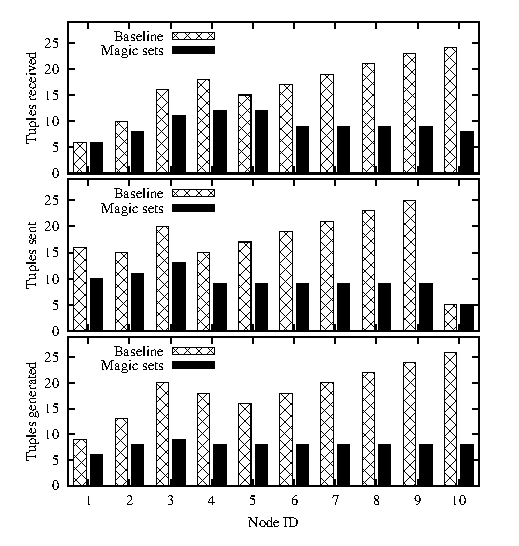
\includegraphics{figures/magicNumbers}
\ssp
\caption{For each node (node ID on $x$ axis), number of tuples received
  (top), sent (middle), and locally generated (bottom) on the $y$ axis.}
\label{ch:evita:fig:magicresults}
\end{figure*}

Figure~\ref{ch:evita:fig:magicresults}(a) shows the number of tuples that each
node receives from the network.  The magic-sets rewritten program causes no
more tuples to be received than the original, and for most nodes significantly
fewer when moving to nodes farther away from the clique.  That is because many
paths that are generated in the original program with destinations within the
clique other than node $node1$ are pruned early on and never transmitted all the
way to the far end.  Similarly, Figure~\ref{ch:evita:fig:magicresults}(b) shows
the number of tuples each node transmits.  Again, the magic-rewritten program
does a lot better.  The two programs have similar tuple transmit/receive
overheads for nodes represents the number of tuples a node sends out over the
network.  

The inclusion of the magic-sets rewrite reduces the number of sends in all but
one case ($node10$).  We note here that the \ol{link}s beyond $node4$ are
directed.  As a result, $node10$ is the only node with no incoming links and is
therefore never burdened with network traffic other than its own.  As a result,
though its received tuple overhead benefits from magic-sets, its transmitted
tuple overhead is unaffected, since it already sends out no extraneous paths
other than its own path to other nodes.  Finally, tuple storage is impacted
beneficially by magic sets everywhere
(Figure~\ref{ch:evita:fig:magicresults}(c)), since both \ol{path} tuples
received from the network, and those generated locally for local consumption
are pruned away by the rewrite.



